\documentclass[a4paper]{article}

\usepackage[T1]{fontenc}
\usepackage{ProfLycee}
\useproflyclib{ecritures}
\usepackage{math-vh}
\usepackage{eurosym}
\usepackage[table]{xcolor}

\usetikzlibrary{matrix,decorations.pathreplacing, calc, positioning,fit}

% *** Réglage des headers ***
\fancyhead[L]{MEXP -- Lycée Victor Hugo}
\fancyhead[R]{Année 2024--2025}
% *** Réglage des headers ***

\begin{document}

\begin{center}
  {\scshape\LARGE Chapitre 5 --- Calcul matriciel\par}
  \vspace{2cm}
\end{center}



\section{Introduction}

\emph{Bien que le calcul matriciel proprement dit n'apparaisse qu'au début du XIXe siècle, les matrices, en tant que tableaux de nombres, ont une longue histoire d'applications à la résolution d'équations linéaires. Le texte chinois Les Neuf Chapitres sur l'art mathématique, écrit vers le IIe siècle av. J.-C., est le premier exemple connu de l'utilisation de tableaux pour résoudre des systèmes d'équations, introduisant même le concept de déterminant. }\\

\emph{En 1545, Jérôme Cardan fait connaître cette méthode en Europe en publiant son Ars Magna. Le mathématicien japonais Seki Kōwa utilise indépendamment les mêmes techniques pour résoudre des systèmes d'équations en 1683. Aux Pays-Bas, Johan de Witt représente des transformations géométriques à l'aide de tableaux dans son livre de 1659, Elementa curvarum linearum. Entre 1700 et 1710, Leibniz montre comment utiliser les tableaux pour noter des données ou des solutions, et expérimente plus de 50 systèmes de tableaux à cet effet. En 1750, Gabriel Cramer publie la règle qui porte son nom. }\\


\begin{example}{}{}
	
Afin de fabriquer des vêtements, on utilise du tissu, du fil et des boutons.\\

Les tableaux ci-dessous récapitulent les quantités nécessaires pour coudre une robe, une chemise ou un jean, ainsi que les prix par fourniture. 


\begin{center}

	\begin{tabular}{cc}
	\begin{minipage}{10cm}
			\begin{tabular}{c|*{3}{C{2cm}|}}
				\hhline{~---}
					&\cellcolor{Red!50} Tissu (en $m$) 	&\cellcolor{Red!50} Longueur de fil (en $m$) & \cellcolor{Red!50} Nombre de boutons\\ \hline
				\multicolumn{1}{|c|}{\cellcolor{Red!50} Robe}				&2,7			&	1,50		& 3\\ \hline
				\multicolumn{1}{|c|}{\cellcolor{Red!50} Chemise} 				& 1,70 		& 	0,70	& 5 \\ \hline
				\multicolumn{1}{|c|}{\cellcolor{Red!50} Jean} 					&		1,50	&	0,50		& 1 \\ \hline
			\end{tabular}
	\end{minipage}
	&
	\begin{minipage}{6cm}
			\begin{tabular}{C{3cm}|*{1}{c|}}
				\hhline{~-}
					&\cellcolor{Red!50} Prix (en \euro)\\ \hline
				\multicolumn{1}{|C{3cm}|}{\cellcolor{Red!50} Tissu au mètre}				&9,95 \\ \hline
				\multicolumn{1}{|C{3cm}|}{\cellcolor{Red!50} Longueur de fil (au $m$)} 				& 1,99 \\ \hline
				\multicolumn{1}{|C{3cm}|}{\cellcolor{Red!50} Bouton (à l'unité)} 					& 0,50 \\ \hline
			\end{tabular}		
	\end{minipage}\\
	
	\end{tabular}


	

		
		\end{center}


%\begin{center}
%\includegraphics[scale=0.9]{01.ps}
%\includegraphics[scale=0.9]{02.ps}
%\end{center}

\bigskip

On peut résumer chacun des tableaux en ne conservant que les nombres. On obtient alors différents tableaux de nombres appelés matrices, notées ici M et P.

On a alors: $M=\begin{pmatrix}
2,70 & 1,50 & 3 \\
1,70 & 0,70 & 5 \\
1,50 & 0,50 & 1 
\end{pmatrix}$ \quad et \quad $P=\begin{pmatrix}
9,95 \\
1,99 \\
0,50 
\end{pmatrix}$

\medskip

\begin{itemize}[label=\textbullet]
	\item M est une matrice possédant autant de lignes que de colonnes. On dit que M est une matrice carrée. Elle est ici de taille 3.

	\item P est une matrice formée d'une unique colonne. On dit que P est une matrice colonne. 
\end{itemize}

\bigskip

\begin{enumerate}
	\item 
	\begin{enumerate}
	\item Calculer le prix de fabrication d'une robe. Faire de même pour une chemise et un jean.
	\item Résumer les résultats obtenus en une matrice colonne T, contenant une ligne pour chaque article en conservant l'ordre robe, chemise, puis jean. 
	
	On admet que l'on peut écrire $M \times P = T$
	\end{enumerate}
	\item On souhaite fabriquer dix robes, dix chemises et dix jeans.
	\begin{enumerate}
		\item Écrire la matrice N contenant trois lignes et trois colonnes pour résumer les quantités nécessaires à cette nouvelle fabrication. 
		\item Quelle opération peut-on conjecturer entre M et N ? 
	\end{enumerate}
\end{enumerate}

\end{example}


\newpage


Dans tout le chapitre $n$ et $m$ désigneront des entiers naturels non nuls

\section{Définitions}

\begin{definition}{}{}
	Une \textbf{matrice} de \textbf{taille} $n \times p$ (ou de format $(n,\,p)$ est un \textquote{\textbf{tableau}} de nombres ayant $n$ lignes et $p$ colonnes. Ce tableau est délimité par des parenthèses (ou des crochets).

\end{definition}


\begin{definition}{}{}
Une matrice $A$ à $n$ lignes et $p$ colonnes est un tableau comportant $n$ lignes et $p$ colonnes.


\begin{minipage}{9cm}
On note $A=(a_{ij})$ où $a_{ij}$ est le \textbf{coefficient} de la $i$-ème ligne et de la $j$-ème colonne.
\end{minipage}

\begin{center}

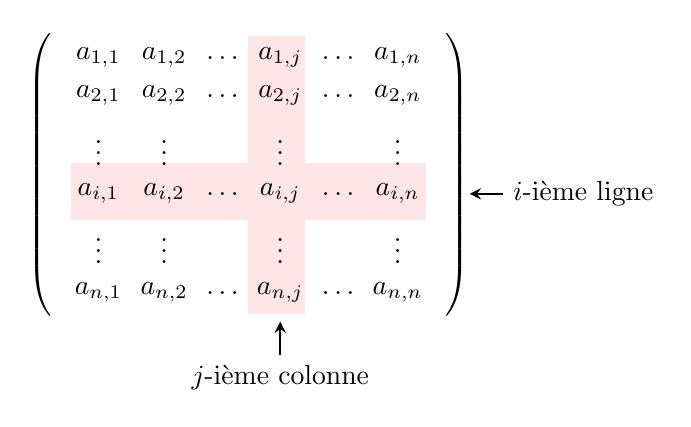
\begin{tikzpicture}[scale=0.7,>=stealth,thick,baseline,
every right delimiter/.append style={name=rd},
]

\draw[fill= Red!10, Red!10] (-3.2,-0.8)--(-3.2,0.2)--(3.2,0.2)--(3.2,-0.8)--cycle;
\draw[fill=Red!10,Red!10] (0,-2.5)--(1,-2.5)--(1,2.5)--(0,2.5)--cycle;

\matrix [matrix of math nodes, 
    left delimiter=(, 
    right delimiter=),
    ](A){ 
a_{1,1} & a_{1,2} & \dots  & a_{1,j} & \dots & a_{1,n}\\
a_{2,1} & a_{2,2} & \dots  & a_{2,j} & \dots & a_{2,n}\\  
\vdots  & \vdots  &  & \vdots  &  & \vdots\\
a_{i,1} & a_{i,2} & \dots  & a_{i,j} & \dots & a_{i,n}\\
\vdots  & \vdots  &  & \vdots  &  & \vdots\\
a_{n,1} & a_{n,2} & \dots  & a_{n,j} & \dots & a_{n,n}\\
};

\draw[<-] (rd.east|-A-4-1.center)--++(0:6mm) node[right]{$i$-ième ligne};
\draw[<-] (A.south-|A-1-4.center) --++(-90:6mm) node[below]{$j$-ième colonne};

\end{tikzpicture}

%\includegraphics[scale=0.4]{2021-08-03_222047.ps}
\end{center}
	
\end{definition}

\begin{example}{}{}
	
\begin{itemize}[label=\textbullet]
	\item $A=\begin{pmatrix}
2 & -3 \\
0 & \dfrac{1}{3} \\
\pi & \sqrt{7} 
\end{pmatrix}$ est de taille $\ldots\ldots\ldots$ et $B=\begin{pmatrix}
0 & 0 & 1 \\
1 & 1 & 0 
\end{pmatrix}$ est de taille $\ldots\ldots\ldots$

\item Si $a_{ij}$ sont les coefficients de $A$, on a par exemple, $a_{12}=\ldots\ldots$, $a_{21}=\ldots\ldots$, $a_{31}=\ldots\ldots$ et $a_{13}$ n'existe pas.
\end{itemize}


\end{example}



\bigskip
\begin{definition}{}{}

\begin{itemize}[label=\textbullet]
	\item Si $n=1$, on dit que $M$ est une \textbf{matrice ligne} formée d'une seule ligne
	\item Si $p=1$, on dit que $M$ est une \textbf{matrice colonne} formée d'une seule colonne
	\item Si $n=p$, on dit que $M$ est une \textbf{matrice carrée d'ordre} $n$
	\item \textbf{Une matrice diagonale} est une matrice carrée d'ordre $n$ dont tous les termes sont nuls sauf ceux qui sont dans la diagonale. 
	\item La \textbf{matrice identité} d'ordre $n$ est une matrice carrée diagonale dont les coefficients diagonaux sont égaux à 1. On la note $I_n$
	\item La \textbf{matrice nulle} de taille $n\times p$ notée $O_{n,p}$ est la matrice de taille $n \times p$ dont tous les coefficients sont nuls.
\end{itemize}	
\end{definition}

\bigskip
\begin{example}{}{}
	
\begin{itemize}[label=\textbullet]
	\item $\begin{pmatrix}
2 & -3 & 1 
\end{pmatrix}$ est une matrice $\ldots\ldots\ldots$ et $\begin{pmatrix}
2\\
-3 \\
1 
\end{pmatrix}$ est une matrice $\ldots\ldots\ldots$

	\item $\begin{pmatrix}
2 & -3 \\
0 & 1  
\end{pmatrix}$ est une matrice $\ldots\ldots\ldots\ldots\ldots\ldots$	et $\begin{pmatrix}
2 & 0 & 0 \\
0 & 3 & 0 \\
0 & 0 & 4 
\end{pmatrix}$ est une matrice $\ldots\ldots\ldots\ldots\ldots\ldots$
\item $\begin{pmatrix}
1 & 0 & 0 \\
0 & 1 & 0 \\
0 & 0 & 1
\end{pmatrix}$ est la matrice $\ldots\ldots\ldots\ldots\ldots\ldots$ et $\begin{pmatrix}
0 & 0 & 0 \\
0 & 0 & 0 \\
0 & 0 & 0
\end{pmatrix}$ est la matrice $\ldots\ldots\ldots\ldots\ldots\ldots$
\end{itemize}

\end{example}

\newpage

\begin{definition}{}{}
	Deux matrices $A$ et $B$ de taille $n\times p$ sont \textbf{égales} lorsque pour tout $i\in [\![1;n]\!]$ et pour tout $ j\in  [\![1;p]\!]$, on a $a_{ij}=b_{ij}$

$$A=B \iff \forall i\in [\![1;n]\!], \forall j\in  [\![1;p]\!], \; a_{ij}=b_{ij} $$ 
\end{definition}

\begin{definition}{}{}
	Une matrice carrée d'ordre $n$ est \textbf{symétrique} lorsque pour tout $i\in [\![1;n]\!]$ et pour tout $ j\in  [\![1;p]\!]$, on a $\ldots\ldots\ldots$
\end{definition}


\bigskip

\begin{example}{}{}
	La matrice $\begin{pmatrix}
\ldots & \ldots & \ldots \\
\ldots & \ldots & \ldots \\
\ldots & \ldots & \ldots
\end{pmatrix}$ est symétrique.
\end{example}



\section{Opérations sur les matrices}

\subsection{Somme et différence}

\begin{definition}{}{}
	On considère deux matrices $A$ et $B$ de même taille.

\begin{itemize}[label=\textbullet]
	\item On définit la \textbf{somme} de $A$ et $B$, notée $C=A + B$ comme la matrice obtenue en additionnant terme à terme les coefficients des matrices $A$ et $B$ (i.e. les coefficients ayant mêmes indices)
	
	On a alors $$\forall (i;j) \in [\![1;n]\!]\times [\![1;p]\!], \, c_{ij}=a_{ij}+b_{ij}$$
	
	\item On définit de la même manière la \textbf{différence} de matrices.
	
	 
\end{itemize}
\end{definition}


\begin{propriete}{}{}
	Soient $A$, $B$ et $C$ trois matrices de mêmes tailles.

\begin{itemize}[label=\textbullet]
	\item \textbf{Commutativité} de la somme de matrice: $A+B=B+A$
	\item \textbf{Associativité} de la somme de matrice: $A+(B+C)=(A+B)+C$
	\item \textbf{Élément neutre} pour l'addition et la soustraction de matrices: $A_{n,m}+O_{n,m}=A_{n,m} $
\end{itemize}
\end{propriete}


\subsection{Produit d'une matrice par un réel}

\begin{definition}{}{}
	Soit $k$ un réel et $A$ une matrice. On définit la matrice $kA$ comme la matrice obtenue en multipliant chaque coefficient de A par $k$. Elle de même taille que $A$.
\end{definition}


\begin{example}{}{}
	Si $A=\begin{pmatrix}
1 & -6 & 5 \\
2 & 4 & -1 
\end{pmatrix}$ et $k = 3$ alors $kA=3A=\begin{pmatrix}
	\ldots & \ldots & \ldots \\
	\ldots & \ldots & \ldots 
\end{pmatrix}$

\end{example}

\begin{definition}{}{}
	Soit $A$ une matrice, on appelle \textbf{opposée} de $A$ la matrice $(-1)A$ notée $-A$. Elle est de même taille que $A$ et formée des coefficients opposés de ceux de $A$

\end{definition}
\begin{propriete}{}{}
	Soient $A$ et $B$ des matrices de même taille $n\times p$ et $k$ et $k'$ deux réels.

$$k(A+B)=kA+kB \qquad (k+k')A=kA+k'A \qquad k(k'A)=(kk')A \qquad  1 \times A = A $$
\end{propriete}


\begin{exercices}{}{}
	20-21-43
\end{exercices}

\begin{exercice}{}{}
On considère les matrices $A=\begin{pmatrix}
4&-1 \\
2&0 \\
-2 & -1 
\end{pmatrix}$ et $B=\begin{pmatrix}
2&2 \\
-3&1 \\
0 & -1 
\end{pmatrix}$
\begin{enumerate}
	\item Calculer $C=3A$ et $D=2B$
	\item Calculer $E=C-D$
	\item Calculer $F=6A+4B$
	\item Déterminer les matrices X de taille $3 \times 2$ telles que $2X+C=A$ 
\end{enumerate}
\end{exercice}

\subsection{Produit de deux matrices}

\subsubsection{Produit d'une matrice par une matrice colonne}

\begin{definition}{}{}
	Soient $A$ une matrice de taille $n \times p$ et $B$ une matrice colonne de $p$ lignes. La matrice $AB$ est définie par:

$$A \times B = (c_{i1}) \quad \text{où} \quad  c_{i1}= a_{i1}b_{1i}+a_{i2}b_{2i}+\ldots + a_{ip}b_{pi}= \sum_{k=1}^{p}\,a_{ip}b_{pi}$$
\end{definition}

\begin{example}{}{}
	Effectuer le produit matriciel entre $A=\begin{pmatrix}
-2 & 1 \\
4 & -1 \\
1 & 0
\end{pmatrix}$ et $B=\begin{pmatrix}
5 \\
-1
\end{pmatrix}$
\end{example}
\subsubsection{Produit de deux matrices}

\begin{definition}{}{}
	Soient $A=(a_{ij})$ et $B=(b_{jk})$ deux matrices telles que le nombre de colonnes de $A$ soit égale au nombre de lignes de $B$ la matrice $AB$ est la matrice définie par:

$$A \times B=(c_{ij}) \quad \text{où} \quad  c_{ij}=a_{i1}b_{1j}+a_{i2}b_{2j}+\ldots + a_{ip}b_{pj}=\sum_{k=1}^{p} \, a_{ik} \times b_{kj}$$
\end{definition}

\bigskip

\begin{example}{}{}
	\begin{minipage}{6cm}
$\begin{pmatrix}
1 & 2 \\
3 & 4 \\
5 & 6 
\end{pmatrix}
\begin{pmatrix}
1 & 2 & 3 \\
4 & 5 & 6
\end{pmatrix}=
$
\vspace{6cm}
\vfill
\end{minipage}
\begin{minipage}{12cm}
\begin{center}

% l' unite
\newcommand{\myunit}{1 cm}
\tikzset{
    node style sp/.style={draw,circle,minimum size=0.3cm},
    node style ge/.style={circle,minimum size=0.3cm},
    arrow style mul/.style={draw,sloped,midway,fill=white},
    arrow style plus/.style={midway,sloped,fill=white},
}

\begin{tikzpicture}[>=latex,scale=0.8]
% les matrices
\matrix (A) [matrix of math nodes,
				column sep=0cm,
             nodes = {node style ge},
             left delimiter  = (,
             right delimiter = )] at (0,0)
{
  a_{11} & a_{12} & \ldots & a_{1p}  \\
  |[node style sp]| a_{21}
         & |[node style sp]| a_{22}
                  & \ldots
                           & |[node style sp]| a_{2p} \\
  \vdots & \vdots & \ddots & \vdots  \\
  a_{n1} & a_{n2} & \ldots & a_{np}  \\
};

\matrix (B) [matrix of math nodes,
             nodes = {node style ge},
             left delimiter  = (,
             right delimiter = )] at (6*\myunit,6*\myunit)
{
  b_{11} & |[node style sp]| b_{12}
                  & \ldots & b_{1q}  \\
  b_{21} & |[node style sp]| b_{22}
                  & \ldots & b_{2q}  \\
  \vdots & \vdots & \ddots & \vdots  \\
  b_{p1} & |[node style sp]| b_{p2}
                  & \ldots & b_{pq}  \\
};
% matrice résultat
\matrix (C) [matrix of math nodes,
             nodes = {node style ge},
             left delimiter  = (,
             right delimiter = )] at (6*\myunit,0)
{
  c_{11} & c_{12} & \ldots & c_{1q} \\
  c_{21} & |[node style sp,red]| c_{22}
                  & \ldots & c_{2q} \\
  \vdots & \vdots & \ddots & \vdots \\
  c_{n1} & c_{n2} & \ldots & c_{nq} \\
};
% les fleches
\draw[blue] (A-2-1.north) -- (C-2-2.north);
\draw[blue] (A-2-1.south) -- (C-2-2.south);
\draw[blue] (B-1-2.west)  -- (C-2-2.west);
\draw[blue] (B-1-2.east)  -- (C-2-2.east);
\draw[<->,red](A-2-1) to[in=180,out=90]
	node[arrow style mul] (x) {$a_{21}\times b_{12}$} (B-1-2);
\draw[<->,red](A-2-2) to[in=180,out=90]
	node[arrow style mul] (y) {$a_{22}\times b_{22}$} (B-2-2);
\draw[<->,red](A-2-4) to[in=180,out=90]
	node[arrow style mul] (z) {$a_{2p}\times b_{p2}$} (B-4-2);
\draw[red,->] (x) to node[arrow style plus] {$+$} (y)%
    to node[arrow style plus] {$+\raisebox{.5ex}{\ldots}+$} (z)
    to (C-2-2.north west);


\end{tikzpicture}

\end{center}
\end{minipage}

\end{example}



\bigskip

\begin{remark}{}{}
\begin{itemize}
	\item La matrice $AB$ aura pour dimension [nbre de lignes de A] $\times$ [nbre de colonnes de B]
	\item En règle générale, \textbf{le produit matriciel n'est pas commutatif}: $AB \neq BA$
\end{itemize}
	
\end{remark}


\subsubsection{Propriétés}

\begin{propriete}{}{}
Soient $A$, $B$ et $C$ trois matrices de dimensions compatibles et un réel $k$.

\begin{itemize}[label=\textbullet]
	\item \textbf{Associativité} du produit: $A(BC)=(AB)C$
	\item \textbf{Distributivité} du produit sur la somme: $A(B+C)=AB+AC$ et $(A+B)C=AC+BC$
	\item $k(AB)= (kA)B=A(kB)$
	\item \textbf{Élément neutre} de la multiplication: $A \times I_n=I_n \times A =A$
	\item \textbf{Mise à la puissance}. On définit le carré de $A$ noté $A^2$ par $A^2=A \times A$. De manière générale, et pour tout $k \in \N^*$, on définit la puissance $k$-ième de $A$ notée $A^k$ comme le produit de $A$ par elle-même $k$ fois:
	$$A^k=\underbrace{A \times A \times \ldots \times A	}_{k \; fois}$$
\end{itemize}
	
\end{propriete}


\begin{remark}{}{}
	Si $A$ est une matrice carrée non nulle d'ordre $n$, on convient que $A^0=I_n$. Alors on peut définir la puissance $k$ par récurrence: $A^0=I_n$ et pour tout $k\in\N$, $A^{k+1}=A^k \times A$.

\end{remark}

\begin{propriete}{}{}
	Soit $A$ une matrice diagonale d'ordre $n$ dont les coefficients diagonaux sont les $a_{ii}$, avec $i \in [\![1;n]\!] $. Alors pour tout $k\in\N^*$, $A^k$ est la matrice diagonale dont les coefficients diagonaux sont les $a_{ii}^k$, avec $i \in [\![1;n]\!] $.
\end{propriete}


\begin{exercices}{}{}
	22-23-24-25-44
\end{exercices}

\section{Matrice inverse d'une matrice carrée}

\begin{theoreme}{}{}
	Soit $A$ une matrice carrée d'ordre $n$. On dit que $A$ est \textbf{inversible} s'il existe une matrice carrée $B$ d'ordre $n$ telle que $AB=I_n$ et $BA=I_n$. Si tel est le cas alors la matrice $B$ est unique et cette matrice est appelée \textbf{inverse} de la matrice $A$. On la note $A^{-1}$.
\end{theoreme}

\begin{remark}{}{}

\begin{itemize}[label=\textbullet]
	\item Par définition, une matrice et son inverse commutent.
	\item Si $A$ est inversible alors $A^{-1}$ également et $(A^{-1})^{-1}=A$.
	\item La matrice $I_n$ est inversible et $I_n^{-1}=I_n$
	\item Toutes les matrices ne sont pas inversibles, en particulier $O_n$.
\end{itemize}
	
\end{remark}


\bigskip

\begin{exercice}{}{}
	 Montrer que $A=\begin{pmatrix}
3 & -1 \\
2 & 1
\end{pmatrix}$ et $B=\begin{pmatrix}
0,2 & 0,2 \\
-0,4 & 0,6
\end{pmatrix}$ sont inverses l'une de l'autre.

\end{exercice}

\begin{definition}{}{}
	Soit $A=\begin{pmatrix}
a & b \\
c & d
\end{pmatrix}$ une matrice carrée d'ordre 2.

On appelle \textbf{déterminant} de $A$ le réel  $ad-bc$ et on le note $det \, A$.
\end{definition}

\begin{propriete}{}{}
	$A$ est inversible si et seulement si $det \; A \neq 0$ et alors dans ce cas:
$$A^{-1}=\dfrac{1}{ad-bc}\begin{pmatrix}
d & -b \\
-c & a
\end{pmatrix}$$
\end{propriete}

\begin{exercice}{}{}
	 Déterminer si possible les inverses de $A=\begin{pmatrix}
1 & 2 \\
3 & 4
\end{pmatrix}$, 
$B=\begin{pmatrix}
3 & -2 \\
-6 & 4
\end{pmatrix}$, 
$C=\begin{pmatrix}
0 & 1 \\
1 & 1
\end{pmatrix}$

\end{exercice}
\begin{exercices}{}{}
	26-27-66-93
\end{exercices}
 
\section{Écriture matricielle d'un système d'équation}


\begin{example}{}{}
	On considère le système de deux équations à deux inconnues:

$$(S) \; \left \{
\begin{array}{rcl}
3x+4y &=& 1 \\
5x+7y & = & -2 
\end{array}
\right.$$

\begin{enumerate}
	\item Déterminer les trois matrices $A$, $X$ et $B$ telles que le système $(S)$ soit équivalent à $AX=B$.
	\item La matrice $A$ est-elle inversible?
	\item En déduire que le système $(S)$ admet une unique solution que l'on déterminera.
\end{enumerate}

\end{example}


\begin{definition}{}{}
	On considère un système linéaire de $n$ équations à $n$ inconnues.

$$(S) \; \left \{
\begin{array}{ccl}
a_{11}x_1+a_{12}x_2+\ldots + a_{1n}x_n &=& b_1 \\
a_{21}x_1+a_{22}x_2+\ldots + a_{2n}x_n &=& b_2 \\
\vdots & = & \vdots \\
a_{n1}x_1+a_{n2}x_2+\ldots + a_{nn}x_n &=& b_n 
\end{array}
\right.$$


On peut associer à $(S)$ les trois matrices:

$$A=\begin{pmatrix}
a_{11} & a_{12} & \ldots & a_{1n} \\
a_{21} & a_{22} & \ldots & a_{2n} \\
\vdots & \vdots & \vdots & \vdots \\
a_{n1} & a_{n2} & \ldots & a_{nn}
\end{pmatrix}, \qquad X=\begin{pmatrix}
x_1 \\
x_2 \\
\vdots \\
x_n
\end{pmatrix}, \qquad B=\begin{pmatrix}
b_1 \\
b_2 \\
\vdots \\
b_n
\end{pmatrix}$$

appelées respectivement \textbf{matrice des coefficients}, \textbf{matrice des inconnues} et \textbf{matrice des seconds membres} telles que le système $(S)$ soit équivalent à l'égalité matricielle: $$AX=B$$
Cette égalité est appelée \textbf{écriture matricielle} de $(S)$.

\end{definition}


\begin{propriete}{}{}
	Si $(S)$ est un système linéaire dont l'écriture matricielle est $AX=B$ et si $A$ est une matrice carrée inversible alors $(S)$ admet une unique solution donnée par la matrice $$X=A^{-1}B$$
\end{propriete}

\begin{demonstration}{}{}
	Soit $(S)$ un système linéaire d'écriture matricielle $AX=B$ et $A$ inversible.

$$AX=B \iff A^{-1}AX=A^{-1}B \iff I_nX=A^{-1}B \iff X=A^{-1}B$$

\end{demonstration}
\bigskip

\begin{exercice}{}{}
	Résoudre le système $(S)$ de 3 équations à 3 inconnues. On pourra s'aider de la calculatrice pour calculer l'inverse d'une matrice.

$$(S) \; \left \{
\begin{array}{rcl}
x-y+2z &=& 5 \\
2x+y-z &=& 1 \\
-x+2y+z & = &6 
\end{array}
\right.$$
\end{exercice}

\begin{exercices}{}{}
	28-29-51-53-54-88-89-90
\end{exercices}
\end{document}